\documentclass[english,a4paper,12pt]{article}
\usepackage[utf8]{inputenc} %for å bruke æøå
\usepackage{babel}
\usepackage{verbatim} %for å inkludere filer med tegn LaTeX ikke liker
\usepackage[document]{ragged2e}
\bibliographystyle{plain}
\usepackage{amsmath}
\usepackage{ulem}
\usepackage[pdftex]{graphicx}
\usepackage{gensymb}
\usepackage{float}
\usepackage{hyperref}
\usepackage{amssymb}
\usepackage[top=0.6in, bottom=0.8in, left=0.9in, right=0.7in]{geometry}
\usepackage{listings}
\usepackage{color}
\usepackage{tikz}

\usepackage{filecontents}
\begin{filecontents}{mybib.bib}
@book{Prandtl,
   author    = "C. Willert, J. Kompenhans",
   title     = "{PIV} {A}nalysis of {L}udwig {P}randtl's {H}istoric {F}low {V}isualization {F}ilms",
   publisher = "Institute of Propulsion Technology, German Aerospace Center, 51170 Koln, German.
   Institute of Aerodynamics and Flow Technology, German Aerospace Center, 37073 Gottingen, Germany",
   address   = "\url{}",
   year      = "2010"
}
@book{HLPIV,
   author    = "Jostein Kolaas",
   title     = "Getting started with {H}ydrolab{PIV} v1.1",
   publisher = "Department of Mathematics, University of Oslo",
   address   = "\url{}",
   year      = "2017"
}
@book{Luddy,
   author    = "John D. Anderson Jr",
   title     = "Ludwig {P}randtl's {B}oundary {L}ayer",
   publisher = "American Institute of Physics",
   address   = "\url{}",
   year      = "2005"
}
\end{filecontents}
\usepackage{natbib}
\usepackage{bibentry}
\nobibliography*

\title{PIV Project (Jean)}
\author{Shako Farhad in collaboration with Valentyna Pysarieva \& Farnaz Rezvany}
\date{\today}

\begin{document}

\definecolor{codegreen}{rgb}{0,0.6,0}
\definecolor{codegray}{rgb}{0.5,0.5,0.5}
\definecolor{codepurple}{rgb}{0.58,0,0.82}
\definecolor{backcolour}{rgb}{0.95,0.95,0.92}
 
\lstdefinestyle{mystyle}{
    backgroundcolor=\color{backcolour},   
    commentstyle=\color{codegreen},
    keywordstyle=\color{magenta},
    numberstyle=\tiny\color{codegray},
    stringstyle=\color{codepurple},
    basicstyle=\footnotesize,
    breakatwhitespace=false,         
    breaklines=true,                 
    captionpos=b,                    
    keepspaces=true,                 
    numbers=left,                    
    numbersep=5pt,                  
    showspaces=false,                
    showstringspaces=false,
    showtabs=false,                  
    tabsize=2
}
 
\lstset{style=mystyle}

\maketitle

\begin{abstract}
An aerodynamic flow over a body can be divided by two regions; a thin boundary layer near the surface, where friction is dominant, and an normal flow external to the boundary layer, where friction is negligible \cite{Luddy}. The HydroLabPIV software reconstructed the turbulence that we see in the videos from Prandtl's flow experiments. This shows that even images with so much disturbance and noise, can give information about a certain phenomena when you use cross-correlation.
\end{abstract}

\section*{Introduction}
There are many ways to measure fluid motion, one of which is particle image velocimetry (PIV). This is a
non-intrusive optical measurement method, which gives velocity fields resolved in both time and space. The software used has been developed at the University of Oslo and is named HLPIV, or HydrLabPIV \cite{HLPIV}. \\ \bigskip 

We are using HydroLabPIV to cross-correlate two images taken with a high-speed camera. This cross-correlation method is then used to further examine the famous images from Ludwig Prandtl's experiment over 110 years ago \cite{Prandtl}. With the advent of Prandtl's boundary-layer concept, it became possible to quantitatively calculate aerodynamic drag \cite{Luddy}.

\section*{Methods}
The overall perspective set forth by Prandtl in his 1905 paper was straightforward. An aerodynamic flow over a body can be divided by two regions; a thin boundary layer near the surface, where friction is dominant, and an normal flow external to the boundary layer, where friction is negligible \cite{Luddy}. \\ \bigskip

We used the HydrolabPIV software to cross-correlate the images extracted from the video of Prandtl's flow experiments. For the options we just used "setpivopt('savepeaks',true);" and "setpivopt('savepeaks',true,'savedisplacements',true);". So we did not have to bother with subwindow size and search range.


\section*{Results}

\begin{figure}[H]
    \centering
    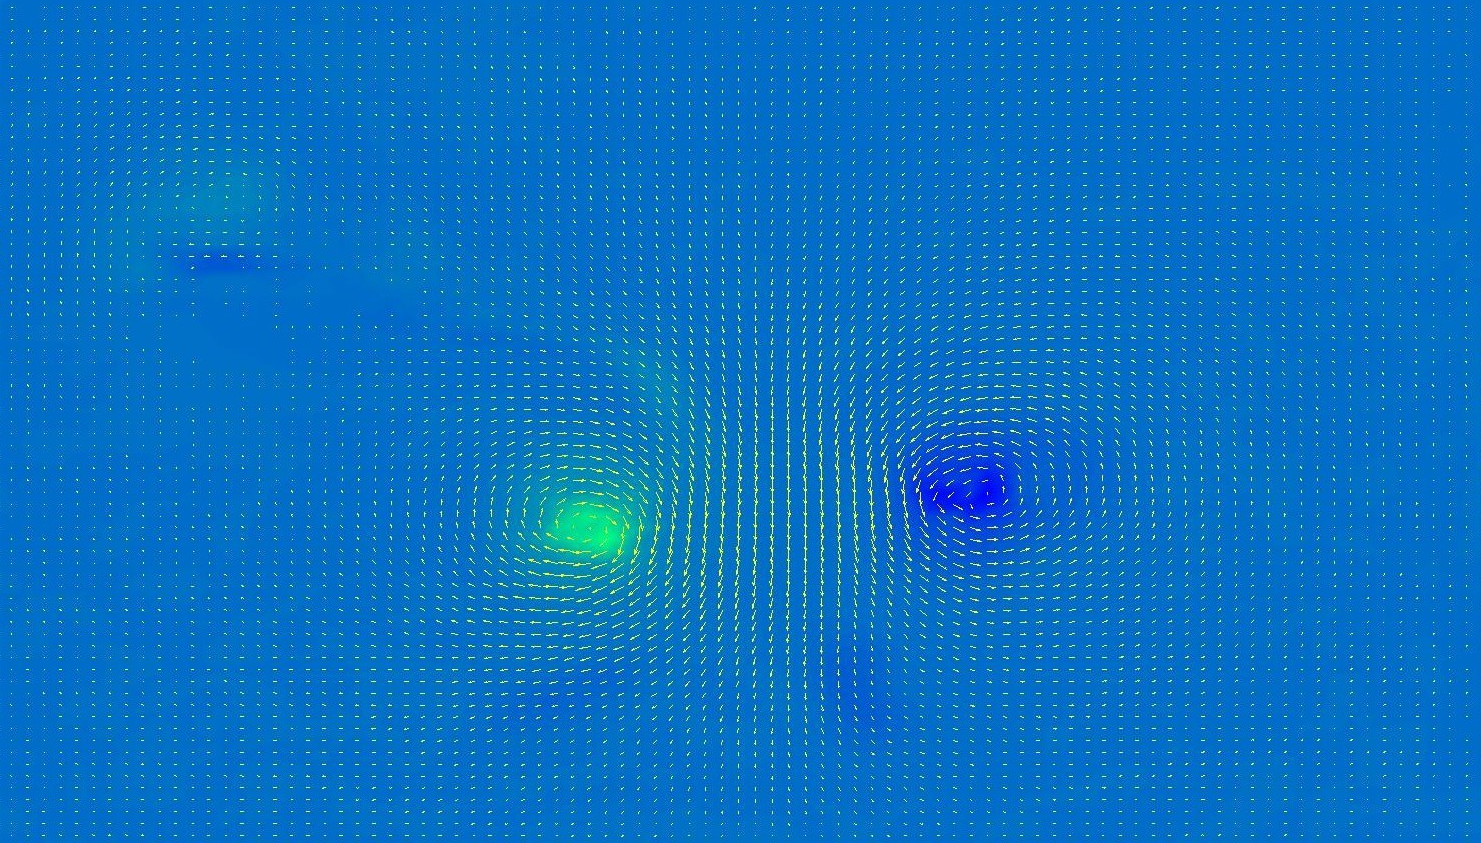
\includegraphics[width=140mm]{seq1.png}
    \caption{Sequence 1: Two vortices that each have opposite spin direction. The one to the right is moving counter-clockwise, and the one to the left is moving clockwise. The "wing" shaped obstacle is barely visible up in the left, but we can see a little bit of whirling taking shape at the front end of the "wing".}
    \label{fig:1}
\end{figure}

\begin{figure}[H]
\centering
\begin{minipage}{.45\textwidth}
    \centering
    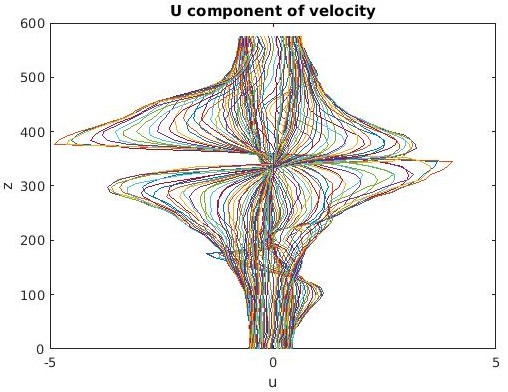
\includegraphics[width=1.1\linewidth]{u_y.jpg}
    \caption{The horizontal velocity component of figure \ref{fig:1} as a function of the height, z. The horizontal velocity is zero right between the two vortices in figure \ref{fig:1}.}
    \label{fig:2}
\end{minipage}%
\hspace{1cm}
\begin{minipage}{.45\textwidth}
    \centering
    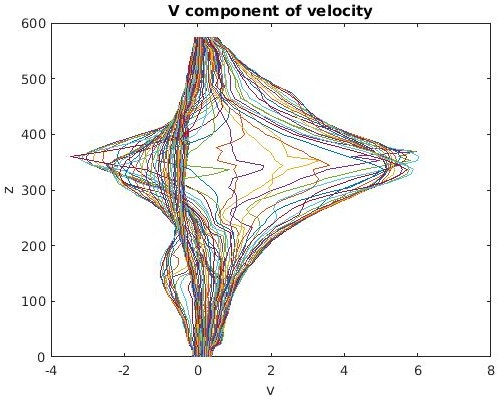
\includegraphics[width=1.1\linewidth]{vmotz.jpg}
    \caption{The veritcal velocity component of figure \ref{fig:1} as a function of the height, z. The horizontal velocity is at its maximum right between the two vortices in figure \ref{fig:1}.}
    \label{fig:3}
\end{minipage}
\end{figure}

\begin{figure}[H]
    \centering
    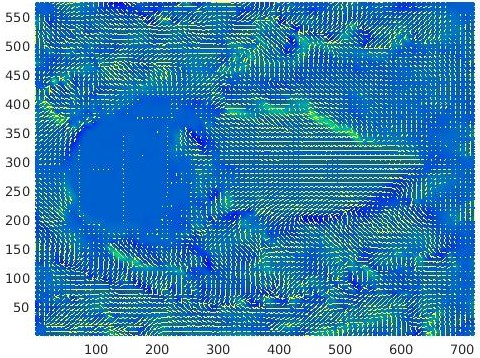
\includegraphics[width=140mm]{sek2.jpg}
    \caption{Sequence 2: A cylinder is placed to the left and turbulence is forming to the right of it.}
    \label{fig:4}
\end{figure}

\begin{figure}[H]
    \centering
    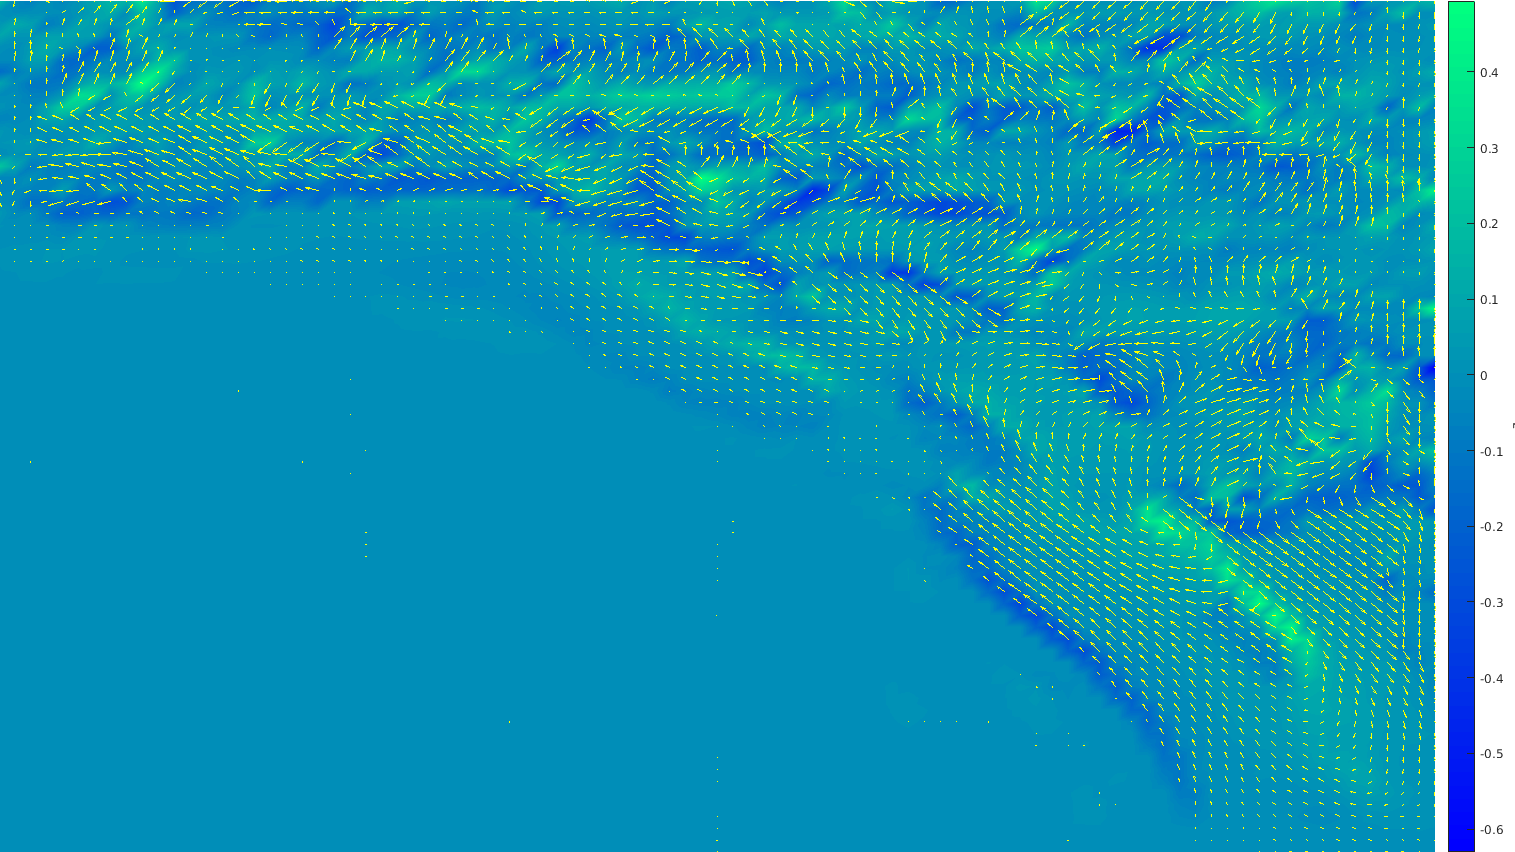
\includegraphics[width=140mm]{sek3.png}
    \caption{Sequence 3: A round shaped object is placed in the fluid and after some time a lot of turbulence is created due to the friction from the surface of the object. The fluid was initially moving from top left to right. From the bottom right the fluid start to move against the stream close to the object. This is why we see greater movement at the bottom right, but initially there was little movement there and all of the movement was in the top left.}
    \label{fig:5}
\end{figure}

\begin{figure}[H]
    \centering
    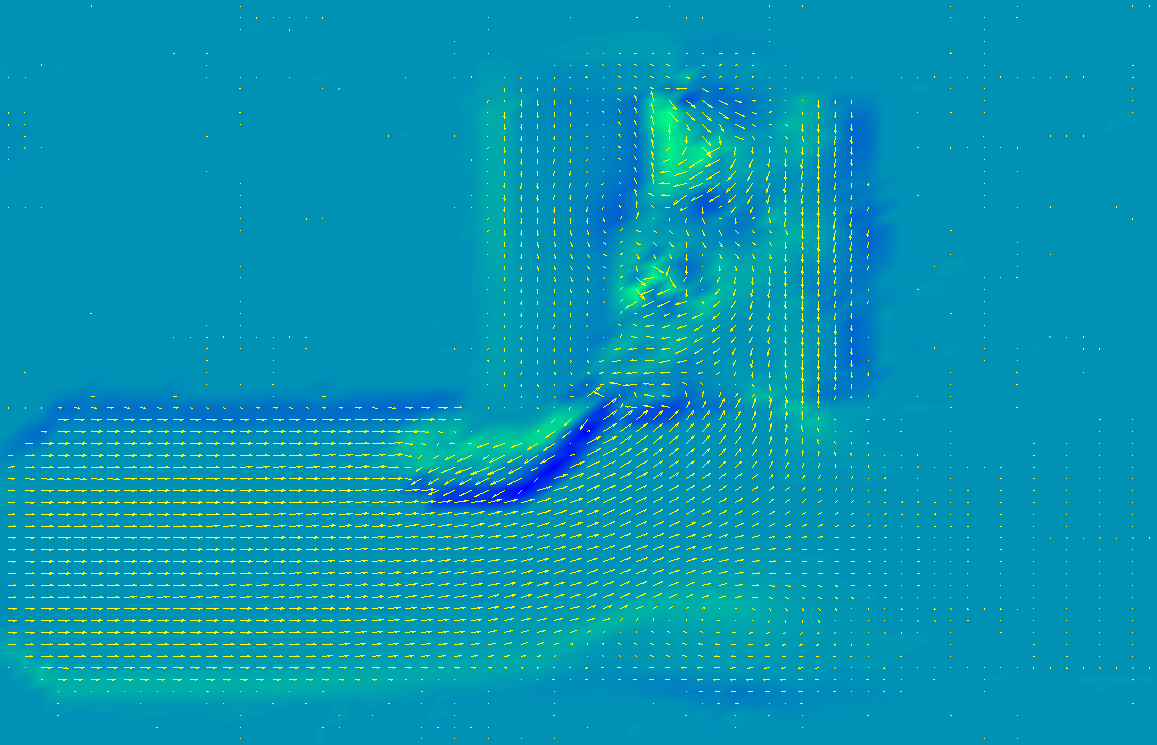
\includegraphics[width=140mm]{sek4.png}
    \caption{Sequence 4: Fluid moving from left to right through pipes with three openings, one to the left, one to the right, and one in the middle at the top. A vortice is forming to the bottom right and this is stopping the fluid from moving to the left, but rather go straight to the top.}
    \label{fig:6}
\end{figure}

\section*{Discussion}
The HydroLabPIV software reconstructed the turbulence that we see in the videos from Prandtl's flow experiments. This shows that even images with so much disturbance and noise, can give information about a certain phenomena when you use cross-correlation. The cross-correlation helped with visualizing the different vortices that were created and to observe the boundary-layer concept. 

\section*{Conclusion}
We were happy with the results, but the program was slow and we spent most of our time just waiting for the results. Of course this was most likely due to the fact that we also did a distortedpass. Hopefully we can make a more efficient program or simply extract information better next time. \\ \bigskip 

We also struggled with understanding why the different vortices were created. We did not know how the different experiments were configured or what made the fluid move in the direction it did. This made us question if it all was friction or if there were other forces at play.

\section*{Appendix}
For matlab code, images and tex source code, see the link below:

\url{https://github.com/ShakoFarhad/PIV-Project-1}

\bibliographystyle{plainnat}
\bibliography{mybib} \bigskip \bigskip
\end{document}
